%!TEX root = Abschluss-ML-Prak-2015.tex
%SEBASTIAN
\section{Ergebnisse}

\subsection{Ergebnisse}

\begin{frame}{Ergebnisse-Regression}
\begin{center}
    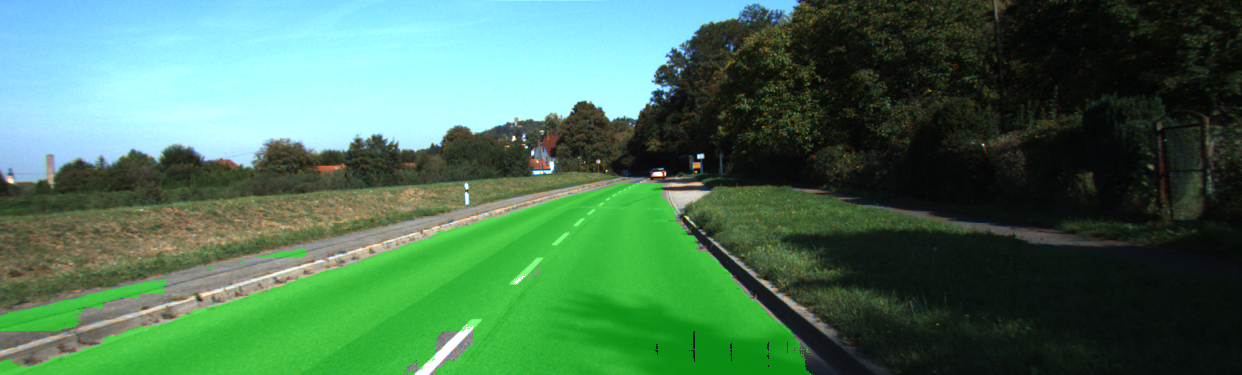
\includegraphics[scale=0.24]{../images/Convolutional/um_000014+-overlay-fully-49-patch.png}
    \vspace{0.1cm}
    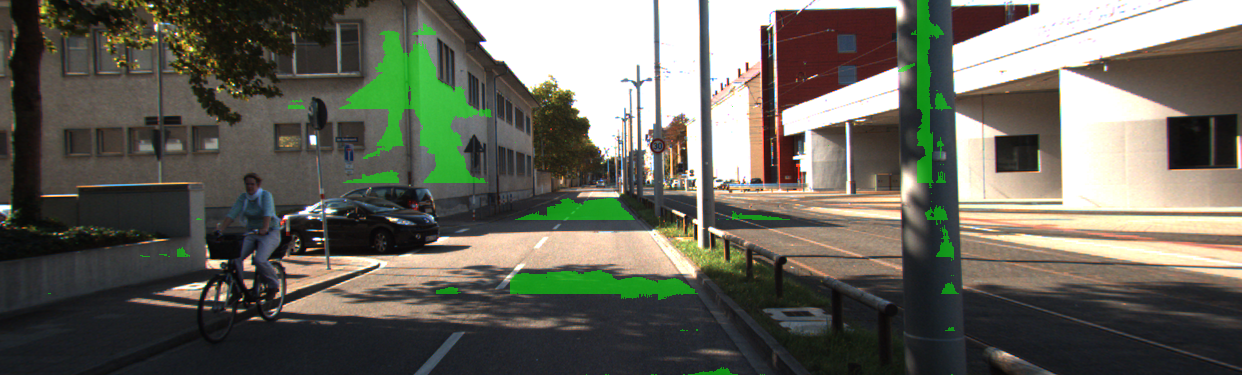
\includegraphics[scale=0.24]{../images/Convolutional/um_000066-overlay-fully-49-patch.png}
        \end{center}
 \end{frame}

\begin{frame}{Vergleich-Klassifikation/Regression}
  \begin{center}
      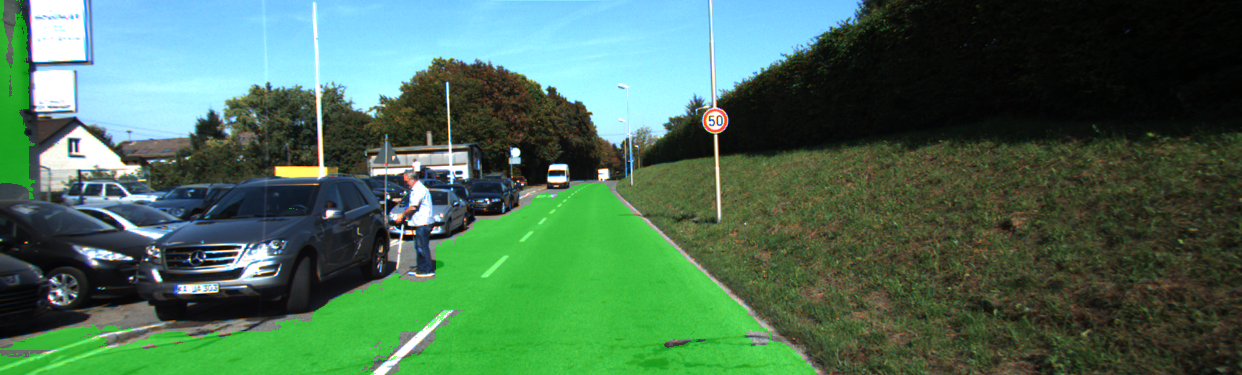
\includegraphics[scale=0.24]{../images/Convolutional/um_000014-overlay-fully-49-patch.png}
         \vspace{0.1cm}
    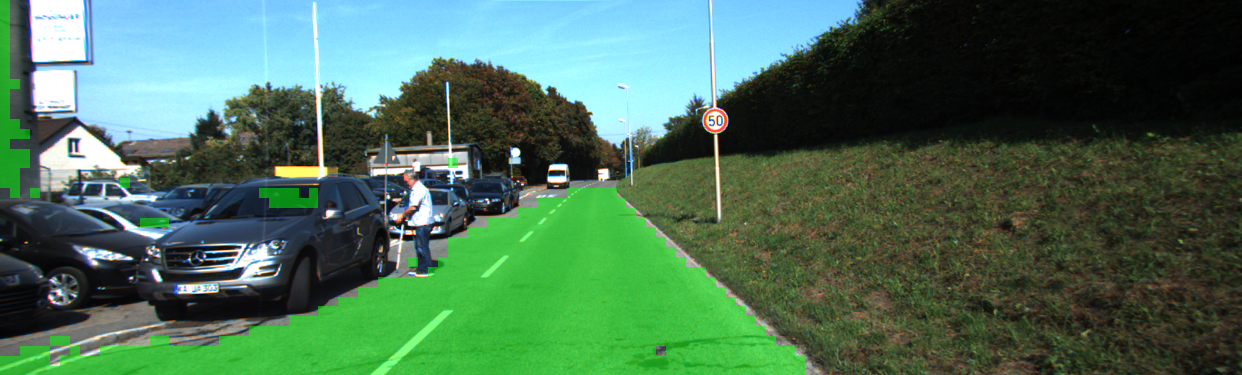
\includegraphics[scale=0.24]{../images/Convolutional/um_000014-overlay.png}
    \end{center}
\end{frame}

\begin{frame}{Bewertung-Klassifikation/Regression}

      
      \begin{table}[h!]
  \begin{center}
   % \caption{Caption for the table.}
    \label{tab:table1}
    \begin{tabular}{c|ccccc}
    \toprule
      \textbf{Netztyp} & \textbf{TN} & \textbf{FP} & \textbf{FN} & \textbf{TP} & \textbf{ACC} \\
       \midrule
      \textbf{Reg. - Stride 10} & 0.977 & 0.022 & 0.197 & 0.802 & 0.947\\
      \textbf{Reg. - Stride 37} & 0.973 & 0.026 & 0.176 & 0.823 &  \textcolor{red}{0.948}\\ 
      \textbf{Reg. - Stride 51} & 0.969 & 0.030 & 0.165 & \textcolor{red}{0.834} & 0.946\\
      \midrule
      \textbf{Kla. - Stride 10} & 0.981 & 0.018 & 0.241 & 0.758 & 0.942\\
      \textbf{Kla. - Stride 37} & 0.959 & 0.040 & 0.212 & 0.787 & 0.929\\
      \textbf{Kla. - Stride 51} & \textcolor{red}{0.982} & 0.017 & 0.451 & 0.548 & 0.906\\
      \bottomrule
    \end{tabular}
    \caption{Ergebnisse der verschiedene neuronalen Netze auf Testset (58 Bilder, ~ 6,7 Mil. Pixel)}
  \end{center}
\end{table}

\end{frame}

\begin{frame}{Laufzeiten-Klassifikation/Regression}

            \begin{table}[h!]
  \begin{center}

  %  \label{tab:table1}
    \begin{tabular}{c|ccc}
    \toprule
      \textbf{Netztyp/Stride} & \textbf{10} & \textbf{37} & \textbf{51} \\
     \midrule
      \textbf{Regression} & 1.99 & 0.29 & 0.18 \\
      \textbf{Klassifikation} & 1.83 & 0.2 & 0.11\\
      \bottomrule
    \end{tabular}
        \caption{Ausf\"uhrungszeit pro Bild (621x188 Pixel) in Sekunden.}
  \end{center}
\end{table}

\end{frame}

\begin{frame}{Video}

      Video

\end{frame}

\section{Ausblick}
\subsection{Ausblick}
\begin{frame}{Ausblick}
    \begin{itemize}
        \item Zu wenig GPU-RAM f\"ur gr\"o\ss ere Patches
        \item Neuronales Netz verbessern
        \item Effizienteres Zusammensetzten der Patches
        \item Mehr Daten (Lense Flare, Beleuchtung, Fahrbahnmakierungen)
    \end{itemize}

\end{frame}